


\documentclass{beamer}
\usetheme{ucl}

\usepackage[utf8]{inputenc}


%%% Increase the height of the banner: the argument is a scale factor >=1.0
%\setbeamertemplate{banner}[ucl][10.0]

%%% Change the colour of the main banner
%%% The background should be one of the UCL colours (except pink or white):
%%%   black,darkpurple,darkred,darkblue,darkgreen,darkbrown,richred,midred,
%%%   navyblue,midgreen,darkgrey,orange,brightblue,brightgreen,lightgrey,
%%%   lightpurple,yellow,lightblue,lightgreen,stone
\setbeamercolor{banner}{bg=darkpurple}
%\setbeamercolor{banner}{bg=yellow,fg=black}

%%% Add a stripe behind the banner
%\setbeamercolor{banner stripe}{bg=darkpurple,fg=black}

%%% The main structural elements
\setbeamercolor{structure}{fg=black}

%%% Author/Title/Date and slide number in the footline
\setbeamertemplate{footline}[author title date]

%%% Puts the section/subsection in the headline
% \setbeamertemplate{headline}[section]

%%% Puts a navigation bar on top of the banner
%%% For this to work correctly, the each \section command needs to be
%%% followed by a \subsection. Requires one extra compile.
% \setbeamertemplate{headline}[miniframes]
%%% Accepts an optional argument determining the width
% \setbeamertemplate{headline}[miniframes][0.3\paperwidth]


%%% Puts the frame title in the banner
%%% Won't work correctly with the above headline templates
%\useoutertheme{ucltitlebanner}
%%% Similar to above, but smaller (and puts subtitle on same line as title)
\useoutertheme[small]{ucltitlebanner}

%%% Gives block elements (theorems, examples) a border
% \useinnertheme{blockborder}
%%% Sets the body of block elements to be clear
% \setbeamercolor{block body}{bg=white,fg=black}

%%% Include CSML logo on title slide
%\titlegraphic{\includegraphics[width=0.16\paperwidth]{csml_logo}}

%%% Include CSML logo in bottom right corner of all slides
%\logo{\includegraphics[width=0.12\paperwidth]{csml_logo}}

%%% Set a background colour
% \setbeamercolor{background canvas}{bg=lightgrey}

%%% Set a background image
%%% Some sample images are available from the UCL image store:
%%%   https://www.imagestore.ucl.ac.uk/home/start
% \setbeamertemplate{background canvas}{%
%   \includegraphics[width=\paperwidth]{imagename}}



%%%%%% Some other settings that can make things look nicer
%%% Set a smaller indent for description environment
\setbeamersize{description width=2em}
%%% Remove nav symbols (and shift any logo down to corner)
\setbeamertemplate{navigation symbols}{\vspace{-2ex}}








\DeclareMathOperator{\Cov}{Cov}
\DeclareMathOperator{\Var}{Var}
\DeclareMathOperator{\E}{\mathbb{E}}
\DeclareMathOperator{\Proba}{\mathbb{P}}

\newcommand{\Covb}[2]{\ensuremath{\Cov\!\left[#1,#2\right]}}
\newcommand{\Eb}[1]{\ensuremath{\E\!\left[#1\right]}}
\newcommand{\Pb}[1]{\ensuremath{\Proba\!\left[#1\right]}}
\newcommand{\Varb}[1]{\ensuremath{\Var\!\left[#1\right]}}

% norm
\newcommand{\norm}[1]{\| #1 \|}

\newcommand{\indep}{\rotatebox[origin=c]{90}{$\models$}}





\usepackage{mathptmx,amsmath,amssymb,graphicx,bibentry,bbm,ragged2e}
\usepackage[english]{babel}

\makeatletter

\newcommand{\noun}[1]{\textsc{#1}}
\newcommand{\jitem}[1]{\item \begin{justify} #1 \end{justify} \vfill{}}
\newcommand{\sframe}[2]{\frame{\frametitle{#1} #2}}

\newenvironment{centercolumns}{\begin{columns}[c]}{\end{columns}}
%\newenvironment{jitem}{\begin{justify}\begin{itemize}}{\end{itemize}\end{justify}}



%\usetheme{Warsaw}
%\setbeamertemplate{footline}[text line]{}
%\setbeamertemplate{headline}{}
%\setbeamercolor{structure}{fg=purple!50!blue, bg=purple!50!blue}

%\setbeamersize{text margin left=15pt,text margin right=15pt}

%\setbeamercovered{transparent}


\@ifundefined{showcaptionsetup}{}{%
 \PassOptionsToPackage{caption=false}{subfig}}
\usepackage{subfig}

\usepackage[utf8]{inputenc}
\usepackage[T1]{fontenc}

\usepackage{multirow}


\makeatother

\def \draft {1}

\usepackage{xparse}
\usepackage{ifthen}
\DeclareDocumentCommand{\comment}{m o o o o}
{\ifthenelse{\draft=1}{
    \textcolor{red}{\textbf{C : }#1}
    \IfValueT{#2}{\textcolor{blue}{\textbf{A1 : }#2}}
    \IfValueT{#3}{\textcolor{ForestGreen}{\textbf{A2 : }#3}}
    \IfValueT{#4}{\textcolor{red!50!blue}{\textbf{A3 : }#4}}
    \IfValueT{#5}{\textcolor{Aquamarine}{\textbf{A4 : }#5}}
 }{}
}
\newcommand{\todo}[1]{
\ifthenelse{\draft=1}{\textcolor{red!50!blue}{\textbf{TODO : \textit{#1}}}}{}
}




\begin{document}


\title[MATSim Sensitivity analysis]{Sensitivity analysis of the MATSim transport model}

\author[Raimbault and Batty]{J.~Raimbault$^{1,2,3,\ast}$ and M.~Batty$^{1}$\\\medskip
$^{\ast}$\texttt{j.raimbault@ucl.ac.uk}
}

\institute[UCL]{$^{1}$Center for Advanced Spatial Analysis, University College London\\
$^{2}$UPS CNRS 3611 Complex Systems Institute Paris\\
$^{3}$UMR CNRS 8504 G{\'e}ographie-cit{\'e}s
}


\date[04/11/2021]{ECTQG 2021\\
Special Session: Exploration and validation of spatial simulation models\\
November 4th 2021
}

\frame{\maketitle}



\section{Introduction}





\sframe{Urban transportation models}{

% The MATSim framework (Multi-Agent Transport Simulation) is a widely used open-source library for such transport simulations, which has been applied to numerous dimensions of transport systems and on many case studies (Axhausen et al., 2016)

\textit{MATSim model: heterogenous data and integration of many sub-models}

\medskip

\begin{center}
	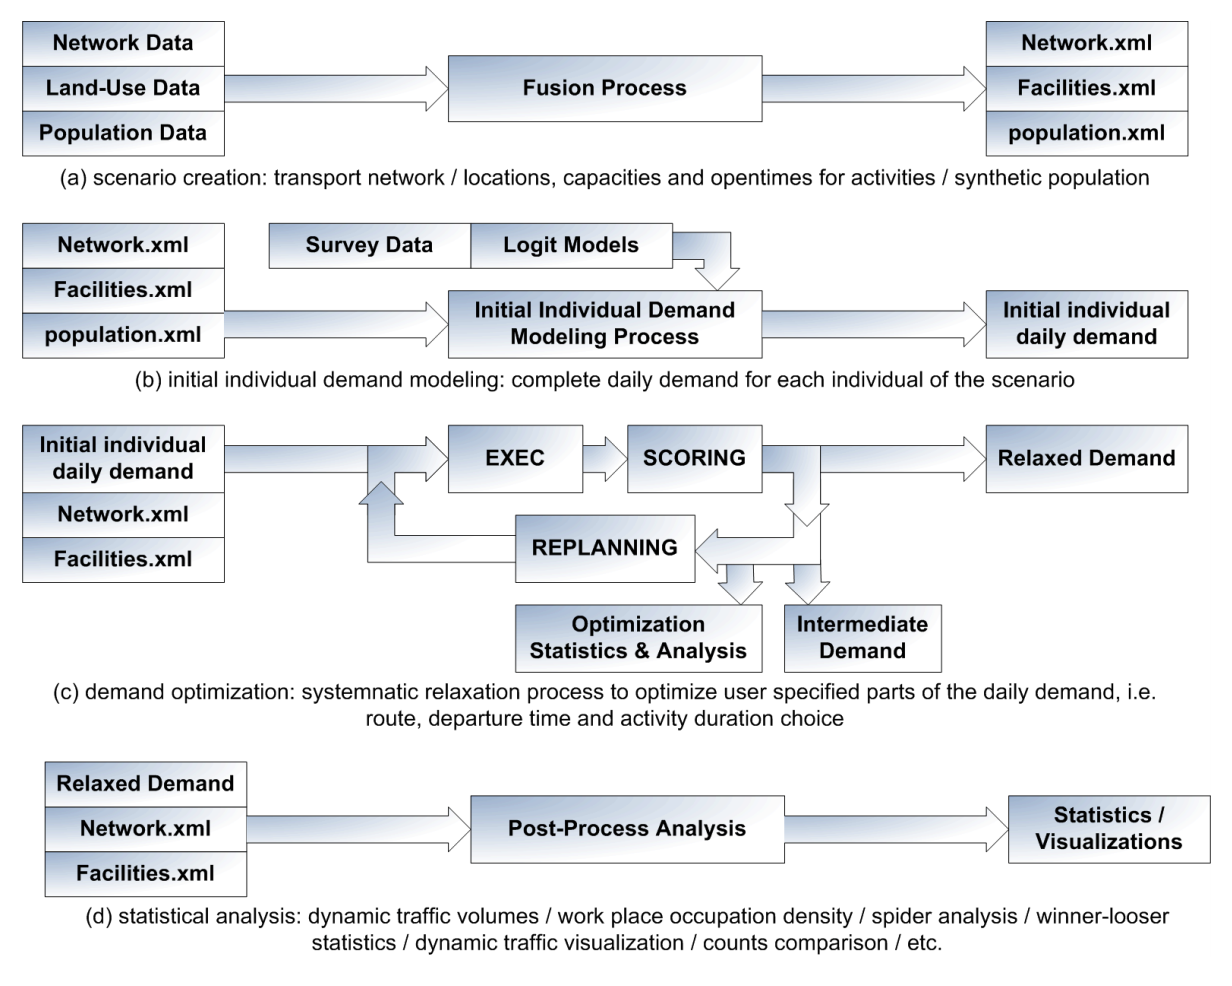
\includegraphics[height=0.7\textheight]{figures/matsim.png}
\end{center}

Source: \cite{balmer2009matsim}

}

\sframe{Land-use transport models}{

\textit{Land-use transport models as a progressive complexification through coupling of detailed sub-models}

\medskip

\begin{center}
	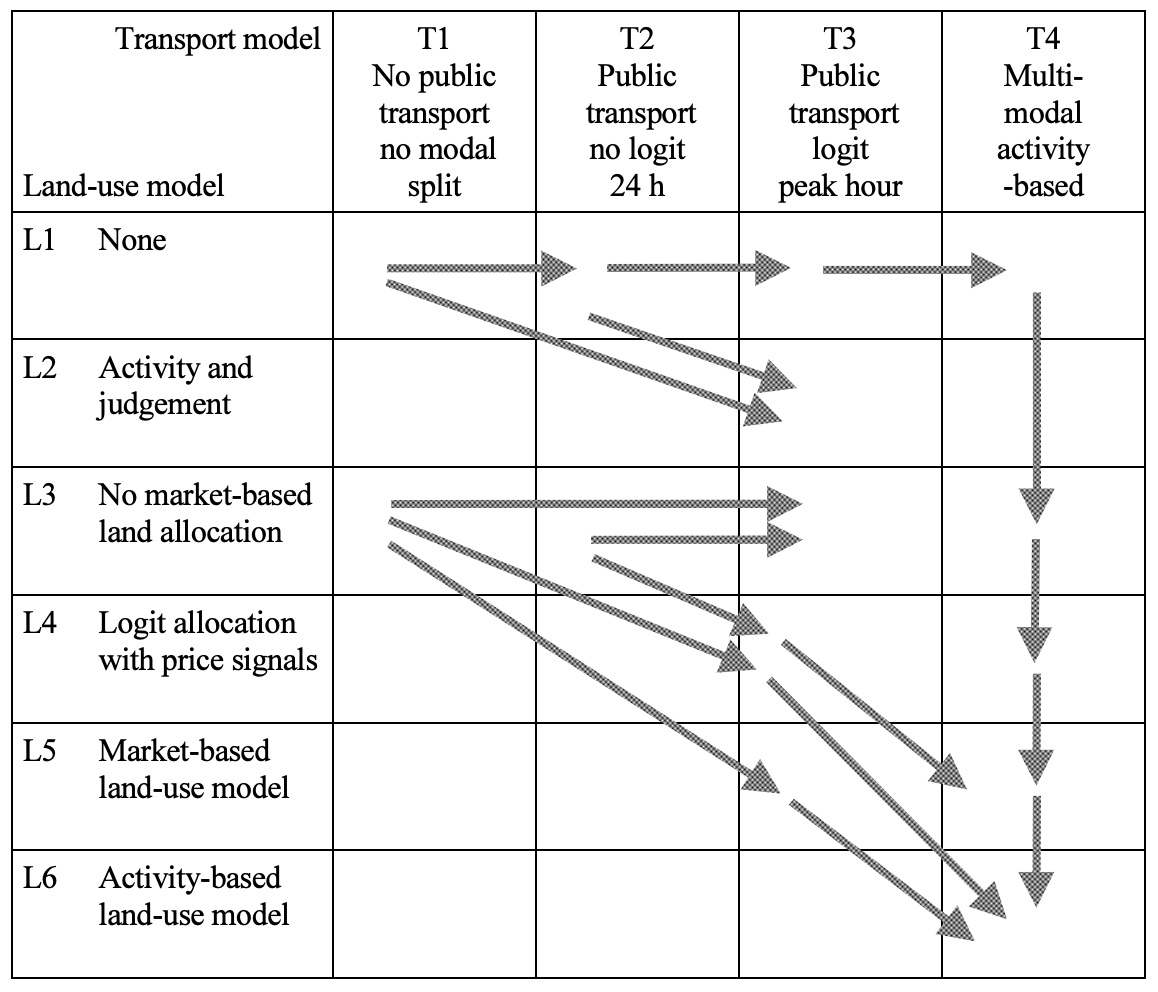
\includegraphics[width=0.45\linewidth]{figures/wegener1.png}\hspace{0.3cm}
	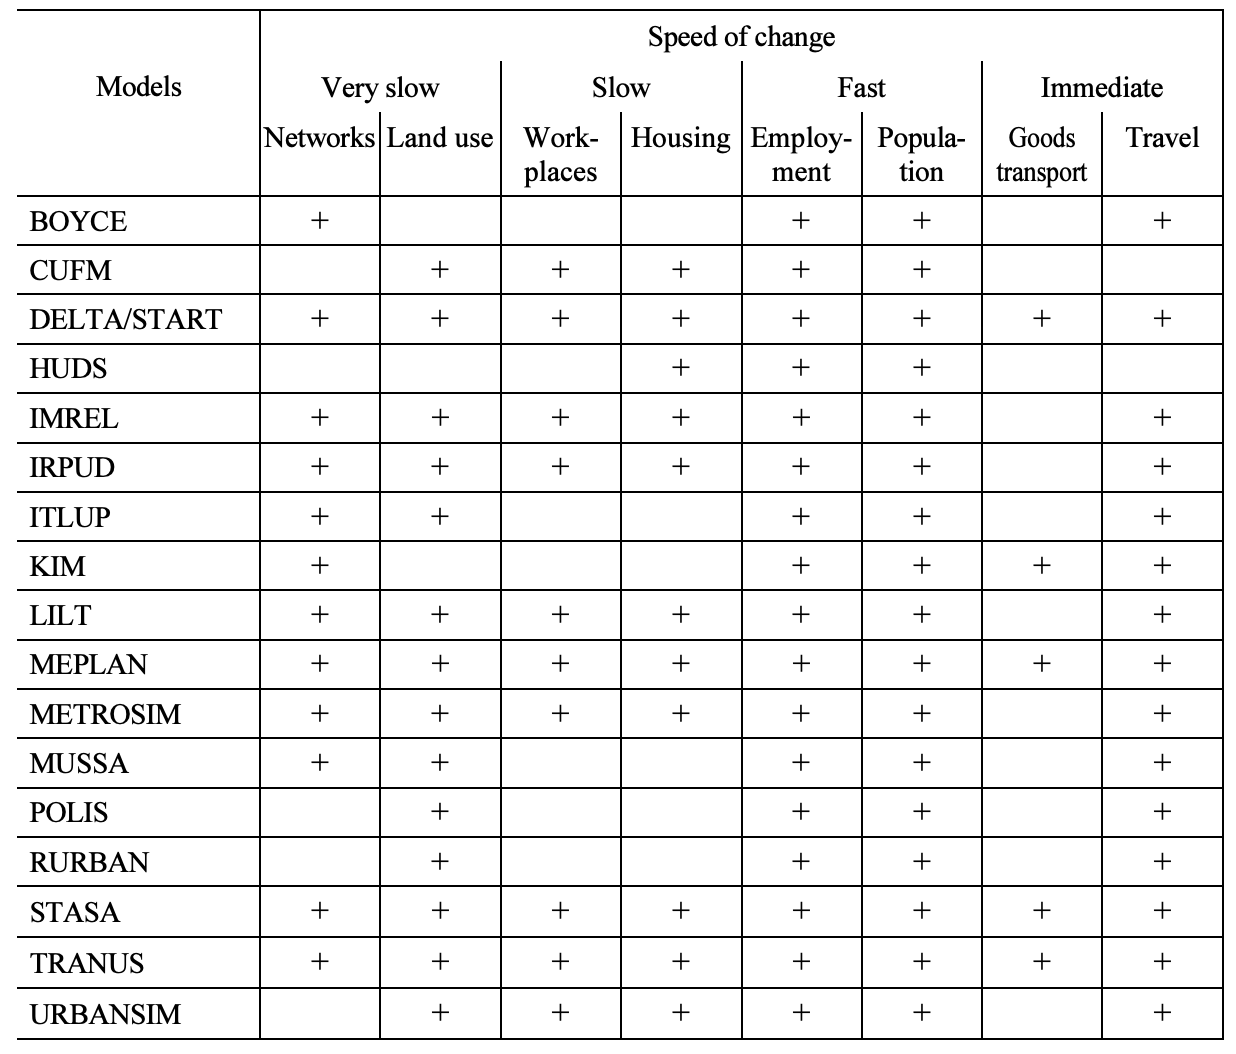
\includegraphics[width=0.45\linewidth]{figures/wegener2.png}
\end{center}

Source: \cite{wegener2004land}

}



\sframe{}{

% Agent-based transport models are useful tools to devise policies related to diverse urban issues, such as long-term urban planning, transport system operations, or health and public transport. In such contexts, a knowledge of result uncertainties and a certain confidence at least in qualitative patterns obtained, is crucial.
% Studies providing some validation and sensitivity analysis of transport models based on MATSim, such as (Zhuge et al, 2019), remain however rare. We contribute in this presentation to the effort of validating these models with a sensitivity analysis of an open data implementation for the UK

\cite{zhuge2019sensitivity}


}






\section{Model}

\sframe{MATSim model integration}{

% We build on the four- step multimodal transport model introduced by (Raimbault and Batty, 2021), which combines, for any urban area in the UK, the generation of synthetic population using the SPENSER model (Lomax and Smith, 2017), spatial interaction modeling integrating the QUANT model (Batty and Milton, 2021), and the MATSim framework.

\textit{Modular four-step multimodal transportation model using open source projects and data}

\bigskip

\textbf{Integrated models:}

\begin{itemize}
	\item MATSim model (MATSim Community) for the transportation system \url{https://www.matsim.org/} \cite{horni2016multi}
	\item SPENSER model (University of Leeds) for the synthetic population \url{https://github.com/nismod/microsimulation}
	\item QUANT model (CASA, University College London) for spatial interactions to generate home-work plans \url{http://quant.casa.ucl.ac.uk/} \cite{batty2021new} % \cite{milton2019accelerating}
	\item spatialdata library (OpenMOLE community) for data processing \url{https://github.com/openmole/spatialdata} \cite{raimbault2020scala}
\end{itemize}



}


\sframe{Data and implementation}{


% Data used to construct the synthetic population is mostly Census data, while transportation networks are built combining Ordnance Survey open data, OpenStreetMap data, and GTFS data for public transport timetables. The QUANT model uses census commuting flows to estimate spatial interaction parameters.

\textbf{Data:}

Generic for any Functional Urban Area (GHSL \cite{florczyk2019ghsl}) or any arbitrary area in the UK: NOMIS census, OrdnanceSurvey roads, Traveline National Dataset for public transport

\medskip

\textbf{Workflow systems:}

\begin{itemize}
	\item DAFNI facility funded by UKCRIC \url{https://dafni.ac.uk}
	\item OpenMOLE software \url{https://openmole.org/} \cite{reuillon2013openmole}
\end{itemize}

\medskip

\textbf{Implementation}

\begin{itemize}
	\item Synthetic SPENSER population distributed at the micro level using OSM buildings
	\item QUANT model to generate home-work commuting flows, job locations determined by sampling flows
	\item Network and plans (simple uniform commuting plans) prepared into MATSim xml files and fed into a multimodal MATSim model
	\item Models integrated as Docker containers
\end{itemize}



}

\sframe{Data preparation}{

$\rightarrow$ Road network preprocessing: implemented into the \texttt{spatialdata} scala library \cite{raimbault2020scala}

\begin{center}
	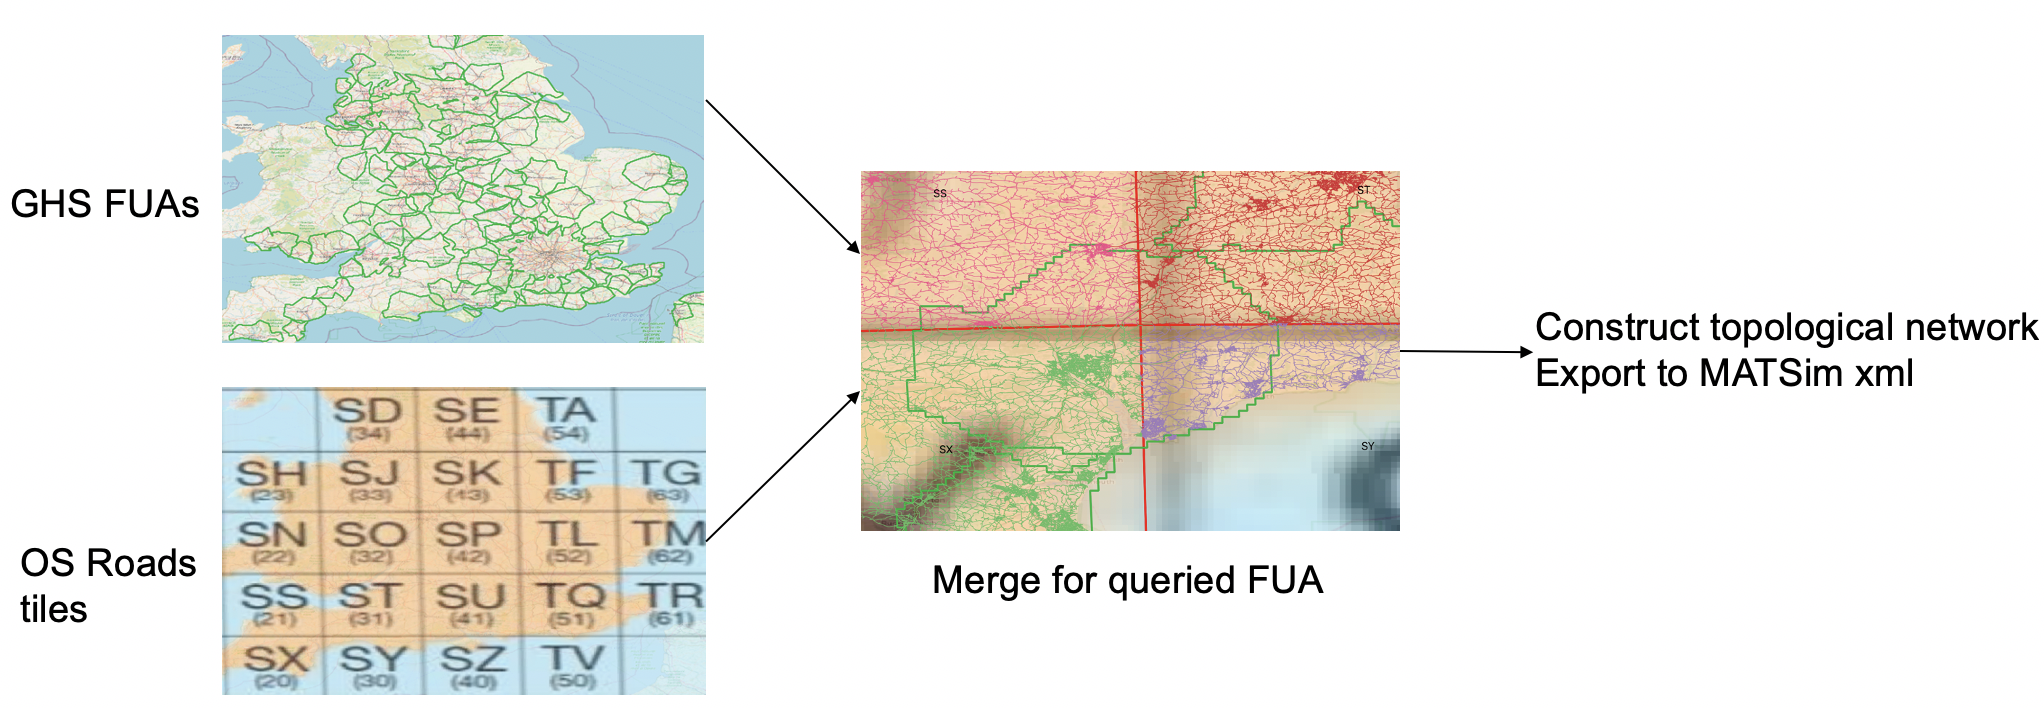
\includegraphics[width=\textwidth]{figures/road_data.png}
\end{center}

\bigskip

$\rightarrow$ Public transport data: from TransXchange (TNDS) to GTFS using UK2GTFS R package \cite{UK2GTFS}; GTFS to MATSim xml schedule using \texttt{pt2matsim} library



}



\sframe{OpenMOLE workflow engine}{



OpenMOLE model exploration open source software \cite{reuillon2013openmole}

\medskip

\begin{center}

\includegraphics[height=0.13\textheight]{figures/iconOM.png}

\includegraphics[height=0.13\textheight]{figures/openmole.png}
\end{center}

\medskip

\textit{Enables seamlessly (i) model embedding; (ii) access to HPC resources; (iii) exploration and optimization algorithms}

\medskip

\url{https://openmole.org/}

}


\sframe{Explored parameters}{

\textit{Parameter sampled for the sensitivity analysis:}

\begin{itemize}
	\item Functional Urban Area (spatial context \cite{raimbault2019space})
	\item Random seed (influence of stochasticity \cite{bienzeisler2021uncertainty}) % gisruk? sds? ewgt!
	\item Synthetic population sampling share
	\item Modal choice parameters \cite{horl2021integrating}: mode constants in scoring function (car, public transport, walking)
\end{itemize}


}




\section{Results}

\sframe{Role of stochasticity}{

\begin{center}
	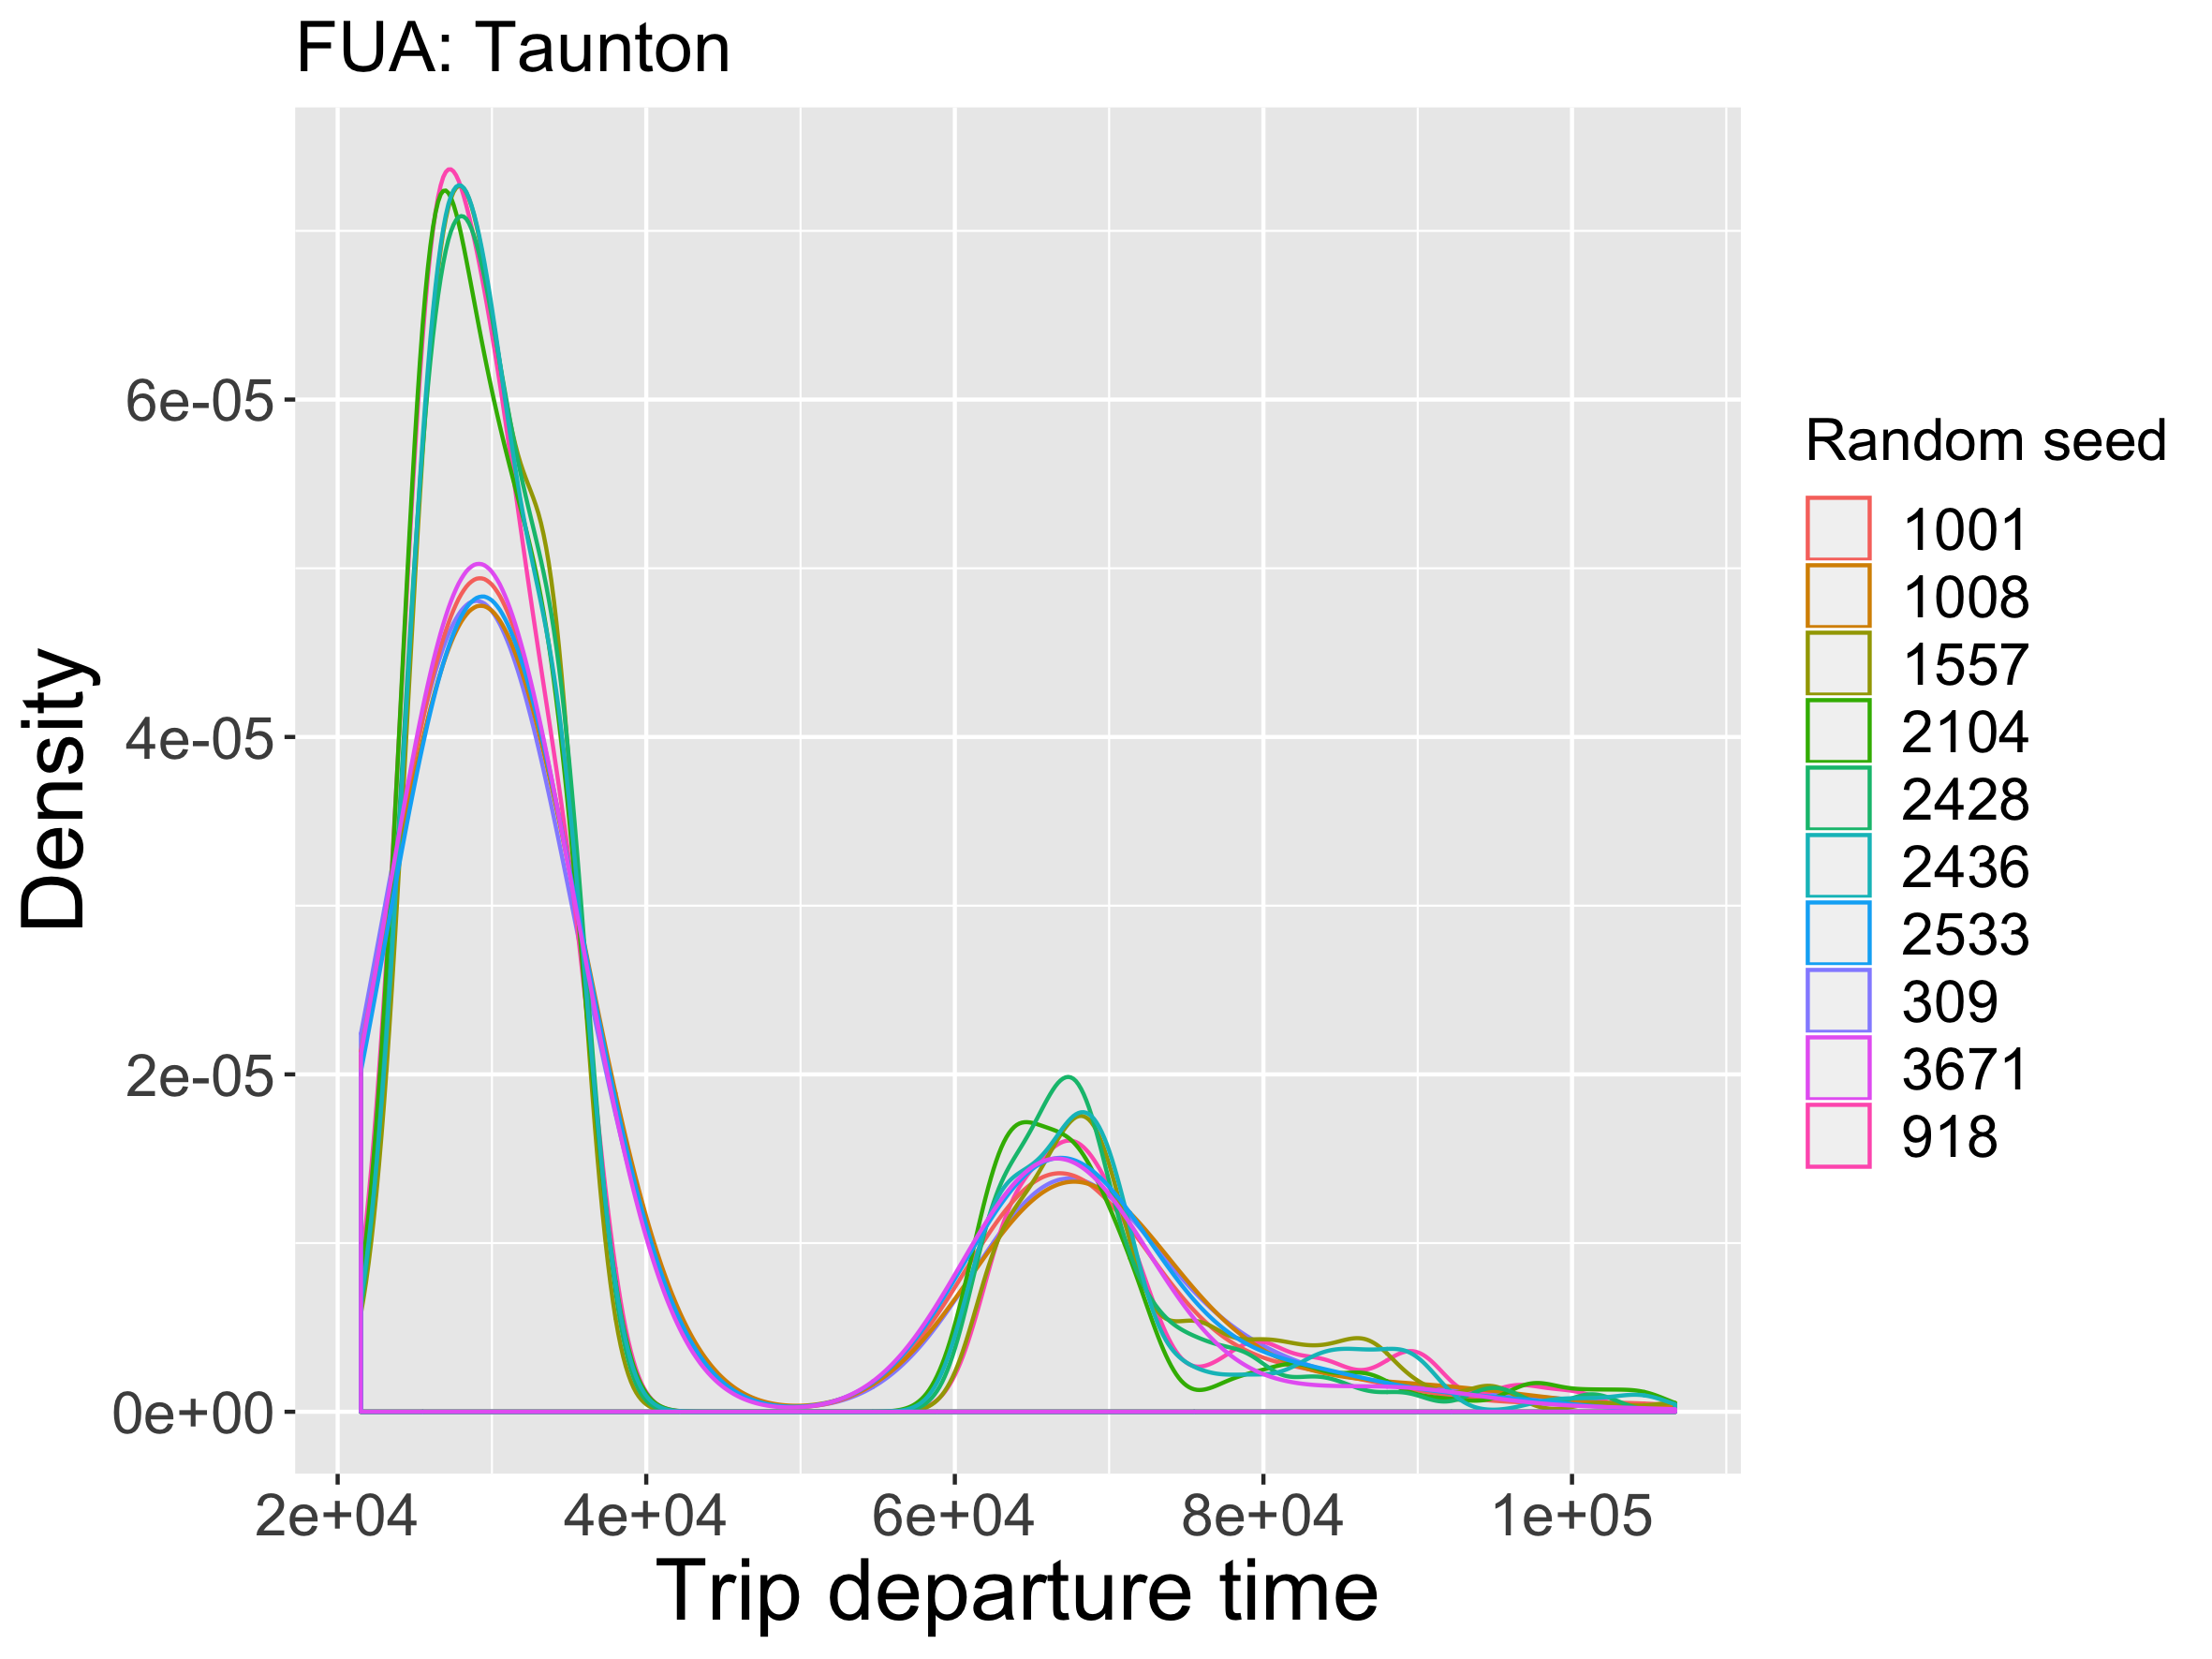
\includegraphics[width=0.9\linewidth]{figures/stochasticity_Taunton.png}
\end{center}


}


\sframe{Global Sensitivity Analysis}{


\textit{Method based on the estimation of conditional relative variances}

\cite{saltelli2010variance}

\medskip

\textbf{First order index}

\[
S_i \textrm{=} \frac{Var \left[ E_{\mathbf{X}_{\sim i}} \left(Y | X_i \right) \right]}{Var\left[Y\right]}
\]

is the expected relative variance reduction if $X_i$ would be fixed

\medskip

\textbf{Total effect index}
\[
ST_i = \frac{E_{\mathbf{X}_{\sim i}}\left[Var(Y | \mathbf{X}_{\sim i}) \right]}{Var(Y)}
\]

is the expected relative variance if all factors but $X_i$ are fixed (includes interaction effects)



}


\sframe{GSA results}{

}




\section{Discussion}



\sframe{Discussion}{

% on reproducibility: still experimental - but totally open. pb of infra? (galere memory e.g.)

% covid? Possible systematic exploration on all urban areas of home-work policies and modifications of agent schedules using genetic algorithms from OpenMOLE
%Visualisation of MATSim agents dynamics (MATSim visu features not open)
% -> role of visualisation?

% Dynamical strong coupling of QUANT and SPENSER to combine population projections with the transport model
% Validation of sub-models and integrated models using advanced model validation methods
% Use MATSim outputs to quantify effective densities in public transport: potential exposure indicators in the COVID-19 context
% Impact of policies and interventions on transport system dynamics and potential contaminations

}





\sframe{Conclusion}{

% Open, reproducible and validated urban models as elementary bricks towards larger integrated models
% Open resource for teaching transport models


\justify

$\rightarrow$ 

\medskip

$\rightarrow$ 

\bigskip
\bigskip



\textbf{Open repositories}

\medskip

\url{https://github.com/JusteRaimbault/UrbanDynamics/Models/Matsim} for containers and workflows

\medskip

\url{https://github.com/openmole/spatialdata} for data processing


\bigskip

\textbf{Acknowledgements}

DAFNI platform/Champions program; Urban Dynamics Lab Grant EPSRC EP/M023583/1

}






%%%%%%%%%%%%%%%%%%%%%
\begin{frame}[allowframebreaks]
\frametitle{References}
\bibliographystyle{apalike}
\bibliography{biblio}
\end{frame}
%%%%%%%%%%%%%%%%%%%%%%%%%%%%










\end{document}





